\chapter{Einleitung}
\label{chap:Intro}
%Die Einleitung liefert eine kurze Einordnung in den Projekthintergrund, um dem
%Leser den Einstieg in die Problemstellung zu ermöglichen. Sie kann je nach Art
%der Arbeit (Literaturrecherche, Konstruktion, praktische Arbeit, etc.) mehr
%oder weniger ausführlich sein, als Richtwert gilt ca. ein bis zwei Seiten.

%Zu den Inhalten der Einleitung zählen:
%
%\minisec{Zielsetzung}
%An dieser Stelle erfolgt die Beschreibung der Aufgabenstellung, Motivation und
%Zielsetzung. Hier wird zunächst das zugrunde liegende Problem bzw. die zugrunde
%liegende Beobachtung erläutert. Anschließend wird auf die wichtigste
%Fragestellung bzw. die eigentliche Forschungsfrage eingegangen, woraus sich
%letztendlich das Ziel und die praktischen Bedeutung der Arbeit ableitet.
%
%\minisec{Stand der Technik}
%Hier wird kurz darauf eingegangen, wo die Aufgabenstellung im aktuellen Stand
%der Technik einzuordnen ist. Dabei werden sowohl bereits geleistete Vorarbeiten
%als auch vergleichbare Tätigkeiten referenziert. Zusätzlich wird hier deutlich
%gemacht, was den Neuheitsgrad dieser Arbeit ausmacht.
%In diesem Kapitel wird zudem kurz umrissen, welche Methoden bisher bekannt
%sind, üblicherweise genutzt werden und inwieweit diese für die gegebene
%Aufgabenstellung von Relevanz sind. Dabei kann bereits eine Bewertung
%hinsichtlich der Zielsetzung erfolgen.
%
%\minisec{Übersicht}
%Zusätzlich soll die Einleitung eine kurze Übersicht über Aufbau und Gliederung
%der Arbeit geben in der kurz beschrieben wird, was in den einzelnen Kapiteln
%bearbeitet wird. Dies dient der Veranschaulichung des Roten Fadens dieser
%Arbeit.

%Die einzelnen Unterpunkte können in einem Fließtext zusammengefasst werden.

Schäden, die durch Stöße verursacht werden sind in vielen technischen
Anwendungen von großer Bedeutung. Vor allem in der Luftfahrt, aber auch in
anderen Bereichen, ist es für die Schadensbeurteilung und Wartungsplanung
wichtig, zu wissen ob Panele und andere zum Teil tragende oder für die Funktion
der Maschine essentielle Komponenten durch einen Stoß beschädigt wurden und
ausgetauscht werden müssen. \\
Im Bereich der Low-Velocity Impacts, welche in dieser Arbeit untersucht werden,
sind die äquivalenten Fälle zum Beispiel ein Werkzeug, das während
Wartungsarbeiten auf den Flügel gefallen ist oder ein Bird-Strike. \\
Hier ist der vorwiegende Parameter die Masse des Stoßobjekts. Es wird vor allem
zwischen High-Mass (hoher Masse) und Low-Mass (niedriger Masse) unterschieden.
(CITATION NEEDED)\\
\\
Da die Masse hier eine zentrale Rolle spielt, wollen wir genauer auf die
Kriterien eingehen: \\
Laut der Gleichung für kinetische Energie: 
\begin{equation}
E = \frac{1}{2}mv^2
\end{equation}
wobei: 
\begin{table}[h!]
	\begin{center}
		\caption{Variablen}
		\label{tab:Tabelle 1}
		\begin{tabular}{l|c}
			\textbf{Variable} & \textbf{Bedeutung}\\
			\hline
			E & Kinetische Energie in Joule\\
			m & Masse in kg\\
			v & Geschwindigkeit in m/s\\
		\end{tabular}
	\end{center}
\end{table}\\
geht die Masse nur mit der ersten Potenz, die Geschwindigkeit andererseits mit
der zweiten Potenz in die Energie ein. Hieraus ist leicht zu erkennen, dass die
Geschwindigkeiten im Low-Velocity Impact Bereich eine gegenüber der Masse
insignifikante Rolle spielt. \\
In der durchgeführten Parameterstudie werden unter anderem der Einfluss der
Stoßstelle, des Gewichts der Stoßmasse und das Material und die Dimensionen der
Platte untersucht. \\
Für das Verständnis des Lesers werden im Folgenden zuerst der aktuelle Stand der
Technik ausgeführt, bevor die physikalischen und mathematischen Grundlagen und
Modelle auf denen das Skript basiert erläutert werden.\\
(Rest der Einleitung dann wenn die Arbeit soweit steht)
\\
\section{Zielsetzung}
Da in vielen Bereichen des Transportsektors kritische Komponenten von Zeit zu
Zeit Stößen ausgesetzt werden, liegt ein Bedarf zur Berechnung dieser Stöße und
dere Folgeschäden vor. \\
In dieser Arbeit wird anhand der Berechnungsgrundlagen von Karas und eines
daraus hergeleiteten Skriptes, eine Parameterstudie zur Untersuchung von
Low-Velocity Stößen auf isotropen Platten durchgeführt. \\
Das Ziel dieser Studie ist, zusammenhänge zwischen Parametern, wie dem Stoßort,
Stoßmasse und Plattenmaße, und dem Plattenverhalten herauszuarbeiten. Diese
können dann für die Bestimmung von Schäden und Reparatur-, bzw.
Austauscharbeiten genutzt werden.\\
%hier noch mehr sobald der Hauptteil steht

\section{Stand der Technik}

Stöße auf Platten haben in der Technik seit langem eine stetig wachsende
Wichtigkeit. \\
Bereits 1881 stellt Heinrich Hertz mit seiner Thesis über die Berührung fester
Körper die ersten Grundlagen für die Berechnung von Stößen und deren Folgen vor.
[HERTZ] \\
In seinen Überlegungen postuliert er, dass wenn ein gerundeter Körper auf eine
Platte trifft, sich dieser Verformen muss, da sonst ein Unstetigkeitspunkt
auftritt. In diesem Punkt würde die Spannung ins Unendliche wachsen, denn laut
der Gleichung für Spannung 

\begin{equation}
\sigma = \frac{Kraft}{Fl\ddot{a}che} \rightarrow \infty \; , \; \; f\ddot{u}r \;
die \; Fl\ddot{a}che \rightarrow 0
\end{equation}

würde die Fläche, wenn keine Verformung stattfindet, gegen 0 gehen. Die Drücke
und Deformationen in diesem Hertzschen Kontakt im Körper sind gegen die
außerhalb der Kontaktzone undendlich groß. \\
Zur Vereinfachung der Berechnung stellt Hertz folgende Annahmen auf, die sich in
vielen späteren Thesen zu diesem Thema wiederfinden: 
\begin{itemize}
	\item Der übertragende Druck zwischen den Körpern ist endlich
	\item Die Kontaktflächen beider Körper sind ideal glatt
	\item Die Körper sind beide isotrop und elastisch
	\item Es stellt sich ein strikt senkrechter Druck zwischen den berührenden Teilen ein
\end{itemize}

In diesem Modell werden die beiden Flächen mathematisch in Berührung gebracht und das verwendete Koordinatensystem in die Fläche die tangential zur Berührungsfläche liegt eingebracht. \\

%Grafik hier

Basierend auf den Hertz'schen Berechnungen hat sich dann am Anfang des 20. Jahrhunderts auch Karas [KARAS] mit der Plattentheorie befasst. Auf seinen Berechnungen basiert in großen Teilen diese Arbeit. Sie werden im Theorie-Teil genauer erläutert, weshalb die Autoren hier nicht weiter vertiefen wollen.\\
Auch Wang [WANG et al.] stellten Überlegungen zu dünnen Platten auf. In ihrer These NONLINEAR LARGE-DEFLECTION BOUNDARY-VALUE PROBLEMS OF RECTANGULAR PLATES von 1948 beschreiben sie die Auslenkung die solche Platten unter seitlichem Schub oder normalem Druck erfahren. Bei kleinen Auslenkungen unterliegt die Deformation einer einfachen linearen Gleichung. Sobald die Auslenkung groß wird, fällt die Beschreibung unter die sogenannten Von Kármán'schen Differentialgleichungen, die Wang et al. durch Finite Differenzen gelöst werden.\\
In der zweiten Hälfte des 20. Jahrhunderts richtet sich der Fokus der Forschung eher Laminatplatten. Shivakumar et al. [SHIV] stellen zwei Modelle zur Bestimmung der Einschlagkraft und Dauer bei Low-Velocity Impactversuchen in zirkularen Laminaten auf. \\
Hierbei leiten sie einmal ein Feder-Masse Modell und ein Energiemodell her. \\
Beide Modelle beinhalten hierbei die Plattendeformation, als auch die des Impactors. Die daraus resultierenden Differentialgleichungen wurden durch verschiedene numerische Methoden gelöst. Das Feder-Masse Modell erwies sich hierbei als praktischere Lösung, da sie neben der maximal auftretenden Kraft auch den Kraftverlauf und die Auslenkung wiedergeben kann. \\

%grafik!! Einmal EB einmal SM Modell

Auch Olsson befasst sich mit Impact-Versuchen auf Platten. Allerdings erweitert er die bestehende Theorie mit einem analytischen Modell um Schäden in Laminatplatten, daher anisotropen Platten, die von Stößen von großen Massen verursacht werden. In seinem Aufsatz stellt er außerdem ein Massenkriterion für das Massenverhältnis von Impactor zu Platte auf. [Olsson]\\
Wichtig ist hier, dass bei sehr kleinen Impactmassen die Platte ballistisch reagiert. Dieses Verhalten wird durch Druckwellen durch die gesamte Platte dominiert. Weiterhin unterscheidet Olsson zwischen small Impact-Mass (kleiner Stoßmasse) und large Impact-Mass (großer Stoßmasse). Das Plattenverhalten bei diesen kleinen Stoßmassen wird vor allem durch Scher- und Biegewellen die nicht in Phase laufen beschrieben. Bei Stoßmassen die wesentlich größer als die Plattenmasse sind, wird ein 'quasi-statisches' Verhalten beobachtet. Hier sind die Spannungen, Verformung und maximalen Belastungen ungefähr in Phase. Auch von Interesse ist, dass Stöße von kleineren Stoßkörpern eher Schäden verursachen als große Stoßkörper mit der gleichen kinetischen Energie.\\
Das Massenkriterion stellt Olsson wie folgt dar.\\
Für die kleinen Stoßmassen kombiniert Olsson die Gleichung für die Position der Vorderkante des n-ten Wellenmodus in Polarkoordinaten:

\begin{equation}
	r_{n}(\theta) = \sqrt{\pi}(\frac{2D_{r}(\theta)}{m})^{\frac{1}{4}} (D*l\sqrt{D_{11}D_{22}})^{\frac{1}{4}}\sqrt{nt}
\end{equation}

wobei $D_{r}(\theta)$ die radiale Plattenbiegesteifigkeit in Richtung $\theta$ und $D_{ii}$ die Plattenfestigkeiten darstellen, mit der Gleichung für die Masse der Platte die von dem Stoß beeinflusst wird:

\begin{equation}
	M_{pWelle} = m \pi r_{1}(0^{\circ}) r_{1}(90^{\circ}) = \pi^{2} t_{imp} \sqrt{2mD^{*}}
\end{equation}

und die Gleichung für die größte Plattenmasse $M_{pmax}$, die von Grenzen (HIER EINMAL STEPHAN FRAGEN WAS ER MIT GRENZEN MEINT) unbeeinflusst bleibt. Diese findet man, indem man die kleinere der beiden elliptischen Flächen die durch:

\begin{equation}
	M_{pmax} = m \pi *min\{(\frac{D_{22}}{D_{11}})^{\frac{1}{4}} r_{xmin}^{2} \; , \; (\frac{D_{11}}{D_{22}})^{\frac{1}{4}} r_{ymin}^{2} \}
\end{equation}		
		
beschrieben werden betrachtet. 

\begin{table}[h!]
	\begin{center}
		\caption{Variablen}
		\label{tab:Tabelle 2}
		\begin{tabular}{l|c}
			\textbf{Variable} & \textbf{Bedeutung}\\
			\hline
			$t_{imp}$ & Zeit am Ende des Stoßvorgangs\\
			m & Stoßmasse in kg\\
			$r_{xmin}$ & Distanz vom Stoß bis zur nächsten Grenze in x-Richtung\\
			$r_{ymin}$ & Distanz vom Stoß bis zur nächsten Grenze in y-Richtung\\
		\end{tabular}
	\end{center}
\end{table}

Ein hinreichendes Kriterium für die wellen-kontrollierte Plattenantwort (kleine Stoßmasse) ist, dass die affektierte Plattenmasse bei $t_{imp}$ nicht größer ist als die Masse die beeinflusst wird, wenn die Grenzen erstmals erreicht werden. Die kombinierten Gleichungen liefern dann: 
\begin{equation}
	\frac{M}{M_{pmax}} \leq \frac{M}{M_{pWelle}} \leq 2 \frac{\sqrt{2}}{\pi^{2}} \approx 0.29
\end{equation}

Bei großen Stoßmassen geht Olsson vor, indem er ein Feder-Masse System modelliert, da die Stoßantwort der Platte, für genügend große Stoßzeiten, quasi-statisch ist. Quasi-statisch bedeutet hier, dass die Last und Auslenkung die gleiche Beziehung wie im statischen Fall haben. Durch zusammenfügen der Stoßzeit $t_{imp}$ und der halben Periodendauer des ersten Vibrationsmodus der Platte ergibt sich: 

\begin{equation}
	\frac{M}{M_{pmax}} \gg \frac{1}{4}
\end{equation}

\begin{figure}[h!]
	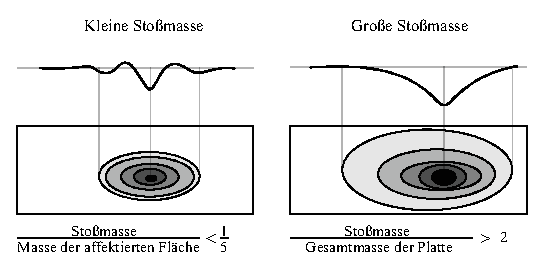
\includegraphics[width=\linewidth]{pictures/einleitung/MassenkriterionOlsson.eps}
	\caption{Massenkriterion nach Olsson}	
	\label{fig:Olsson}
\end{figure}


Zuletzt wollen wir noch auf das Kriterion für mittlere Stoßmassen eingehen. Bei einem zentriertem Stoß auf einer quasi-isotropischen Platte ergibt sich:

\begin{equation}
	\frac{1}{5} < \frac{M}{M_{pmax}} < 2
\end{equation}

Da dieser jedoch für diese Arbeit nicht von großer Relevanz ist, wird hier nicht näher darauf eingegangen.



Im Rahmen der Stoßversuche werden in der aktuellen Forschung vor allem
Untersuchungen mit Laminatverbundsplatten durchgeführt. [Olsson etc]. Hierbei
konzentriert sich ein Großteil der Forschung auf Stöße in der Plattenmitte
[Olsson, Shivakumar etc]. \\
Um das Plattenverhalten während und nach des Stoßes zu beschreiben, wird unter
anderem auf Energie-Masse und Feder-Masse Modelle die von Shivakumar et al.
aufgestellt wurden zurückgegriffen. [Shivakumar] \\
Weitere Modelle wurden von Karas und Olsson hergeleitet, wobei das Modell von
Karas einen Hauptbestandteil dieser Arbeit darstellt. [CITATION NEEDED] Olsson
befasst sich in seiner Arbeit vor allem mit Verbundlaminaten und Delamination
aufgrund von Stößen. \\
Andererseits stellt Karas in seiner Arbeit eine Berechnungsgrundlage für
Stoßvorgänge mit Navierschen Randbedingungen [Vielleicht kurz erklären?] und
einer reduzierten Plattenmasse dar. Die Berechnungen und physikalischen
Grundlagen werden im Theorieteil dieser Arbeit genauer erklärt, weshalb diese
hier nicht weiter vertieft werden.\\
Eine weitere Berechnungsmethode wurde von Reissner und Mindlin entworfen. Diese
ist auch gütlig, wenn die Kirchoff'sche Plattenbedingung nicht anwendbar ist:
\begin{equation}
\frac{Plattendicke}{Seitenl\ddot{a}nge} = \frac{1}{10}
\end{equation}
In der sogenannten Reissner-Mindlin Plattentheorie wird angenommen, dass die
Plattennormale während Deformation nicht orthogonal zur Plattenmittelebene
bleibt. Hierdurch eignet sich diese auch zur Berechnung von
Schubspannungseffekten. [Onate]\\
Da die Berechnung nach Reissner-Mindlin das lösen von Differentialgleichungen
höherer Ordnung erfordert, stellt sie für diese Arbeit nur einen geringen Anteil
dar und wird daher bei Bedarf genauer erläutert. [satz evtl entfernen]\\




